\documentclass[11pt,a4paper]{article}

\usepackage[polish]{babel}
\usepackage[utf8]{inputenc}
\usepackage{polski}
\usepackage[T1]{fontenc}
\usepackage{indentfirst}
\usepackage{wrapfig}    % for wrapping figures, tables

\frenchspacing

%\usepackage{amsmath}
\usepackage{physics}
%\usepackage{bm}
\usepackage{gensymb}
%\usepackage{hepnames}
\usepackage{epsfig}
\usepackage{graphics}
\usepackage[shortlabels]{enumitem}
%\usepackage{xspace}
%\xspaceaddexceptions{[]\{\}}

%
%
%fixpagesize
\pagestyle{empty}
\addtolength{\textwidth}{6cm}
\addtolength{\textheight}{4cm}
\addtolength{\evensidemargin}{-3cm}
\addtolength{\oddsidemargin}{-3cm}
\addtolength{\topmargin}{-2cm}
\parindent=0cm


%
%
%small distance in list/item/enum for enumitem package
\setlist[itemize,enumerate]{topsep=0em}
\setlist{noitemsep}

%print zadanie #
\newcounter{zadanie}\newcommand{\zadanie}[1][]{\addtocounter{zadanie}{1} ~\\  {\bf \emph{Zadanie \arabic{zadanie} #1 }} \\}
\newcounter{zaddom}\newcommand{\zaddom}[1][]{\addtocounter{zaddom}{1} ~\\  {\bf \emph{Zadanie domowe \arabic{zaddom} #1 }} \\}
%\renewcommand{\zadanie}[1][]{\pagebreak  ~\\  {\bf \emph{Zadanie }} \\} \addtolength{\topmargin}{-2cm}

\newcommand{\dbar}{{\mkern3mu\mathchar'26\mkern-12mu d}}


%%%%%%%%%%%%%%%%%%%%%%%%%%%%%%%%%%%%%%%%%%%%%%%%%%%%%%
\begin{document}           % End of preamble and beginning of text.

\begin{centering}
\bf{\Large{Termodynamika z elementami fizyki statystycznej}}\\
Tydzień 7 (6 kwietnia 2020)\\[3mm]
Cykle termodynamiczne, maszyny cieplne\\
\end{centering} 
\vspace{5mm}

\zadanie
Dla teoretycznej maszyny cieplnej, której gazem roboczym jest gaz doskonały, 
i pracującej w oparciu o cykl Carnota, znajdź bezpośrednim rachunkiem:
\begin{enumerate}[a)]
\item sprawność silnika
\item efektywność lodówki
\item efektywność pompy cieplnej
\end{enumerate}
Załóź, że maszyna działa między dwoma zbiornikami o temperaturach 0\degree C i 60\degree C.\\

{\em Rozwiązanie:}
Rozpatrzmy bilans energetyczny dla każdej z przemian.
\begin{itemize}
	\item przemiana izotermiczna $AB$: dla gazu doskonałego $\Delta U = 0$ czyli $\Delta Q = - \Delta W$. Policzmy pracę podczas tej przemiany
	\begin{equation}
		W_{AB} = - \int_{V_A}^{V_B} p {\rm d}V =  n R T_2  \ln \frac{V_A}{V_B} < 0.
	\end{equation}
	czyli
	\begin{equation}
		Q_{AB} = - n R T_2 \ln \frac{V_A}{V_B} > 0.
	\end{equation}
	\item przemiana adiabatyczna $BC$: $\Delta Q = 0$ więc $\Delta U = \Delta W$. Zmianę energii jest łatwo policzyć
	\begin{equation}
		U_{BC} = - n C_V (T_2 - T_1) < 0,
	\end{equation}
	więc 
	\begin{equation}
		W_{BC} = - n C_V (T_2 - T_1) < 0, \qquad Q_{BC} = 0.
	\end{equation}
	\item przemiana izotermiczna $CD$, analogicznie do przemiany $AB$ znajdujemy
	\begin{equation}
		W_{CD} =  n R T_1 \ln \frac{V_C}{V_D} > 0, \qquad Q_{CD} = - n RT_1 \ln \frac{V_C}{V_D} < 0.
	\end{equation}
	\item przemiana adiabatyczna $DA$, analogicznie do przemiany $BC$ znajdujemy
	\begin{equation}
		W_{DA} = n C_V (T_2 - T_1), \qquad Q_{DA} = 0.
	\end{equation}
\end{itemize}
Korzystając z równiania stanu gazu doskonałego i równania adiabaty znajdujemy również, że
\begin{equation}
	\frac{V_C}{V_D} = \frac{V_B}{V_A}.
\end{equation}
Liczymy teraz sprawność i efektywności.
\begin{enumerate}[a)]
	\item sprawność silnika zdefiniowana jest jako uzyskana (przez nas) praca w stosunku do dostarczonego (do gazu) ciepła, czyli
	\begin{equation}
		\eta = \frac{-W_{\rm całk}}{Q_{\rm dost}},
	\end{equation}
	gdzie $W_{\rm całk} = W_{AB} + W_{BC} + W_{CD} + W_{DA}$ jest całkowitą pracą wykonaną nad gazem a $Q_{\rm dost} = Q_{AB}$. Otrzymujemy
	\begin{equation}
		\eta = - \frac{n R T_2 \ln V_A / V_B + n R T_1 \ln V_C / V_D}{- n R T_2 \ln V_A / V_B} = \frac{T_2- T_1}{T_2} = 1 - \frac{T_1}{T_2}.
	\end{equation}
	\item cykl chłodniczy: po pierwsze lodówka działa w cyklu odwrotnym do cyklu silnika więc wszystkie przemiany przebiegają w odwrotną stronę. Efektywność lodówki definiujemy jako ciepło pobrane podzielone przez wykonaną pracę
	\begin{equation}
		\eta = \frac{Q_{\rm pobrane}}{W_{\rm całk.}},
	\end{equation}
	gdzie $Q_{\rm pobrane} = Q_{DC} = - Q_{CD}$, natomiast $W_{\rm całk} = W_{AD} + W_{DC} + W_{CB} + W_{BA}$.
	Po podstawienu dostajemy
	\begin{equation}
		\eta = \frac{T_1}{T_2 - T_1}.
	\end{equation} 
	\item efektywność pompy ciepła zdefiniowana jest jako ilość ciepła oddanego podczas cyklu do wykonanej pracy
	\begin{equation}
		\eta  = \frac{Q_{\rm oddane}}{W_{\rm całk.}},
	\end{equation}
	z $Q_{\rm oddane} = Q_{BA}$. Otrzymujemy
	\begin{equation}
		\eta = \frac{T_2}{T_2- T_1}.
	\end{equation}
\end{enumerate}

%%%%%%%%%%%%%%%%%%%%%%%%%%%%%%%%%%%%%%%
\newpage
%%%%%%%%%%%%%%%%%%%%%%%%%%%%%%%%%%%%%%%


\begin{wrapfigure}[10]{r}{0.3\linewidth}\vspace{0mm}
\resizebox{\linewidth}{!}{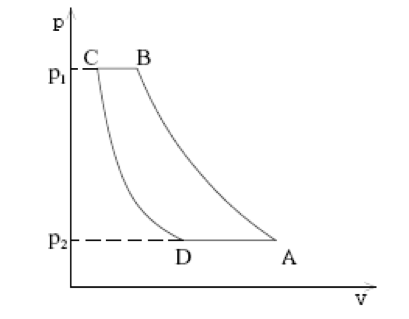
\includegraphics{rys_lodowa.png}}
\end{wrapfigure}
\zadanie
Zbudowano lodówkę działającą w następującym procesie cyklicznym (rysunek): gaz roboczy jest najpierw sprężany izotermicznie w temperaturze otoczenia $T_1$ do ciśnienia $p_1$. Sprężony gaz doprowadzany jest do kontaktu termicznego z wnętrzem lodówki i chłodzony izobarycznie do jego temperatury $T_2$. Następnie, wciąż w kontakcie z wnętrzem lodówki, gaz jest izotermicznie rozprężany do ciśnienia $p_2$. Wreszcie doprowadzany jest z powrotem do kontaktu termicznego z otoczeniem i ogrzewa się izobarycznie do temperatury $T_1$, powracając w ten sposób do stanu początkowego.
Przyjmując, że gaz roboczy jest dwuatomowym gazem doskonałym ($C_p=\frac{7}{2}R$):
\begin{enumerate}
\item Znajdź współczynnik sprawności opisanej lodówki.
\item Oblicz, dla jakiej najniższej temperatury $T_2$ lodówka będzie jeszcze działać przy ustalonych $T_1, p_1$ i $p_2$ (tzn. będzie jeszcze pobierała ciepło ze swego wnętrza).
\end{enumerate}
{\em Wskazówki:}
 \begin{enumerate}
 \item  rozpatrz ciepło pobrane lub oddane i pracę wykonaną przez lub nad gazem roboczym przy przemianach na odcinkach AB i CD (przemiany izotermiczne) i BC i DA (przemiany izobaryczne). Sprawność lodówki jest dana stosunkiem ciepła pobranego netto z lodówki do pracy netto wykonanej nad gazem.  Wynik $\eta=\frac{T_2}{T_1-T_2}-\frac{7}{2\log(p_1/p_2)}$.\\
 \item Ciepło pobrane netto powinno być dodatnie.  Wynik: $T_2\geq \frac{T_1}{1+(R/c_p)\, \times \log(p_1/p_2)}$.
 \end{enumerate}
 
 
{\em Rozwiązanie:}
Żeby policzyć efektywność lodówki musimy znać całkowitą pracę wykonaną przez gaz oraz ilość ciepła pobranego z wnętrza lodówki. Rozpatrzmy szczegółowo pracę i ciepło w 4 procesach
\begin{itemize}
 	\item przemiana izotermiczna $AB$:
	\begin{equation}
		W_{AB} = - n R T_1 \ln \frac{V_B}{V_A}, \qquad Q_{AB} = n R T_1 \ln \frac{V_B}{V_A}.
	\end{equation}
	\item przemiana izobaryczna $BC$:
	\begin{equation}
		W_{BC} = - n R (T_2 - T_1), \qquad W_{BC} = n C_p (T_2 - T_1).
	\end{equation}
	\item przemiana izotermiczna $CD$:
	\begin{equation}
		W_{CD} = - n R T_2 \ln \frac{V_D}{V_C}, \qquad Q_{CD} = n R T_2 \ln \frac{V_D}{V_C}.
	\end{equation}
	\item przemiana izobaryczna $DA$:
	\begin{equation}
		W_{DA} = n R (T_1 - T_2), \qquad Q_{DA} = n C_p (T_1 - T_2).
	\end{equation}
\end{itemize}
 Całkowita praca wykonana przez gaz
 \begin{equation}
 	W = W_{AB} + W_{BC} + W_{CD} + W_{DA} =  n R \left( T_1 \ln \frac{V_A}{V_B} + T_2 \ln \frac{V_C}{V_D} \right).
 \end{equation}
 Gaz jest w kontakcie termicznym z wnętrzem lodówki w czasie przemian $BC$ i $CD$ i całkowite ciepło dostarczone do gazu (czyli pobrane z lodówki) wynosi
 \begin{equation}
 	Q = Q_{BC} + Q_{CD} = n R T_2 \ln \frac{V_D}{V_C} - n C_P (T_1 - T_2).
 \end{equation}
 Korzystając z równania stanu gazu doskonałego możemy wyrazić stosunek nieznanych objętości do stosunku znanych ciśnień
 \begin{equation}
 	\frac{V_D}{V_C} = \frac{p_1}{p_2}.
 \end{equation}
 Lodówka będzie działać dopóki $Q>0$ i korzystając z powyższej relacji oraz ze wzoru na $Q$ otrzymujemy
 
 \begin{equation}
 	T_1 < T_2\left( 1 + \frac{2}{7}\ln \frac{p_1}{p_2} \right).
 \end{equation}

Efektywność lodówki liczymy jako całkowite ciepło pobrane z wnętrza lodówki podzielone przez całkowitą pracę wykonaną przez nas nad gazem,
\begin{equation}
	\eta = \frac{Q}{W} = \frac{T_2}{T_1 - T_2} - \frac{7}{2 \ln p_1/p_2}.
\end{equation}
 
%%%%%%%%%%%%%%%%%%%%%%%%%%%%%%%%%%%%%
\newpage
%%%%%%%%%%%%%%%%%%%%%%%%%%%%%%%%%%%%%%

\zadanie
\begin{wrapfigure}[10]{r}{0.3\linewidth}\vspace{-5mm}
\resizebox{\linewidth}{!}{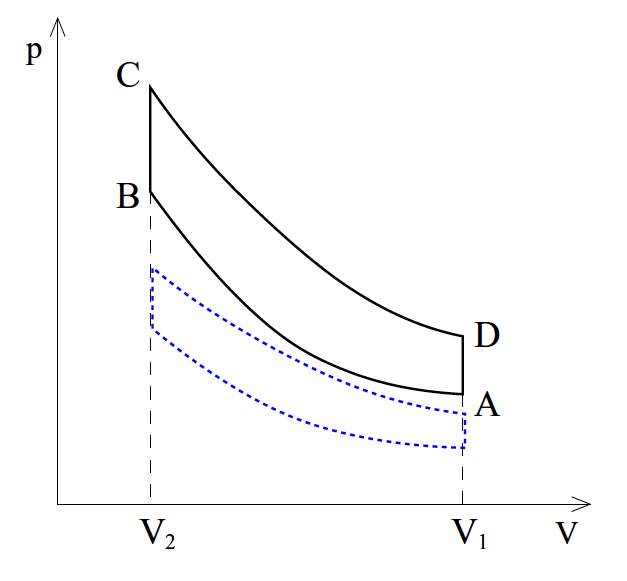
\includegraphics{rys_otto.png}}
\end{wrapfigure}
%
Działanie silnika spalinowego można w przybliżeniu opisać tzw. cyklem
Otto (rysunek). W cyklu tym gaz wypełniający cylinder (mieszanka powietrza z paliwem,
pobrana w cyklu ssania) jest najpierw adiabatycznie sprężany od objętości $V_1$
do $V_2$. W chwili osiągnięcia minimalnej objętości mieszanka jest zapalana. Wydzielone ciepło
powoduje izochoryczny wzrost ciśnienia gazu. Następuje adiabatyczne rozprężenie z powrotem
do objętości początkowej $V_1$. W punkcie tym otwierany jest zawór wydechowy.
Rozprężanie gazu powoduje spadek temperatury. Oblicz sprawność takiego silnika.\\
{\em Wskazówka:}\\  Sprawność silnika jest równa stosunkowi wykonanej pracy do pobranego ciepła w całym cyklu. Skorzystać z równań dla adiabaty, żeby znaleźć relacje między temperaturami na początku i końcu przemiany adiabatycznej. \\
Wynik: sprawność $\eta=1-(V_2/V_1)^{\kappa-1}$, gdzie $\kappa$ jest wykładnikiem adiabaty  $pV^\kappa=const.$


{\em Rozwiązanie:}
W cyklu całkowita zmiana energii wewnętrznej $\Delta U = 0$ więc z I zas. termodynamiki $ \Delta W = - \Delta Q$. Procesy $AB$ i $CD$ są adiabatyczne więc
\begin{equation}
	\Delta Q = Q_{BC} + Q_{DA}.
\end{equation}
Sprawność silnika zdefiniowana jest jako całkowita praca wykonana przez gaz, podzielona przez ciepło dostarczone do gazu
\begin{equation}
	\eta = \frac{- \Delta W}{Q_{BC}} = 1 + \frac{Q_{DA}}{Q_{BC}} = 1 + \frac{T_A - T_D}{T_C - D_A},
\end{equation}
gdzie w ostatnim kroku policzyliśmy ciepła w przemianach izochorycznych. Nieznane temperatury możemy wyrazić przez znane objętości korzystając z równania adiabaty i równania gazu doskonałego
\begin{equation}
	T_A V_1^{\kappa-1} = T_B V_2^{\kappa - 1}, \qquad T_C V_2^{\kappa-1} = T_D V_1^{\kappa - 1}.
\end{equation}
Ostatecznie
\begin{equation}
	\eta = 1 - \left( \frac{V_1}{V_2} \right)^{\kappa - 1}.
\end{equation}

%%%%%%%%%%%%%%%%%%%%%%%%%%%%%%%%%%%%%%%%%
\newpage
%%%%%%%%%%%%%%%%%%%%%%%%%%%%%%%%%%%%%%%%%%

\zadanie
Rozważyć proces cykliczny w którym gaz doskonały najpierw jest izotermicznie rozprężany 
do próżni od objętości $V_A$ do $V_B$, 
następnie izobarycznie ($p=p_0=const$) jest sprężany do objętości $V_A$, 
po czym ogrzewany jest on izochorycznie ($V=V_A=const$) tak, 
iż stan układu wraca do stanu początkowego. 
Jest to cykl Mayera i za jego pomocą wykaż dla gazu doskonałego, że $C_p-C_v=R$.\\

{\em Rozwiązanie:}
Skorzystamy z tego, że dla cyklu $\Delta U = 0$. W procesie izotermicznym $AB$ energia wewnętrzna gazu doskonałego nie zmienia się, więc $U_{AB} = 0$. Policzmy zmianę energii wewnętrznej podczas dwóch pozostałych procesów z I zas. termodynamiki.
\begin{itemize}
	\item proces izobaryczny $BC$. Ciepło $Q_{BC}$ możemy policzyć ponieważ znamy ciepło właściwe $C_p$, natomiast pracę liczymy wprost z definicji, dostajemy
	\begin{equation}
	Q_{BC} = n C_p (T_C - T_B) = \frac{C_p p }{R}(V_C - V_B), \qquad W_{BC} =  p (V_B - V_C).
	\end{equation}
	więc
	\begin{equation}
		U_{BC} = p (V_B - V_C) \left(1 - \frac{C_p}{R} \right).
	\end{equation}
	\item proces izohoryczny $CA$. W procesie izochorycznym praca wynosi $0$, więc $W_{CA} = 0$ i $U_{CA} = Q_{CA}$. Ponieważ znamy ciepło właściwe $C_V$ otrzymujemy,
	\begin{equation}
		U_{CA} = n C_V (T_A - T_C) = n C_V (T_B - T_C) = \frac{p C_V}{R}(V_B - V_C),
	\end{equation}
	gdzie w drugim kroku skorzystaliśmy z tego, że przemiana $AB$ jest izotermiczna.
\end{itemize}
Całkowita zmiana energii wynosi więc
\begin{equation}
	0 = \Delta U = p (V_B - V_C) \left(1 - \frac{C_p}{R} + \frac{C_V}{R} \right),
\end{equation}
z czego wynika, że $C_p - C_V = R$.

%%%%%%%%%%%%%%%%%%%%%%%%%%%%%%%%%%%%%%%%
\newpage
%%%%%%%%%%%%%%%%%%%%%%%%%%%%%%%%%%%%%%%%%

\zadanie
Znajdź sprawność silnika, który działa w oparciu o cykl Carnota między temperaturami 
$T_2$ i $T_1$ ($T_2<T_1$) i w którym substancją roboczą jest gaz fotonowy.\\
{\em Wskazówka:}\\
Dla gazu fotonowego izobara jest jednocześnie izotermą. \\
Wynik: sprawność $\eta=1-\frac{T_2}{T_1}$.

{\em Rozwiązanie:}
Sprawność silnika
\begin{equation}
	\eta = \frac{- W}{Q_{\rm pobrane}} = \frac{Q_{\rm całk}}{Q_{\rm pobrane}} = \frac{Q_{AB} + Q_{CD}}{Q_{AB}} = 1 + \frac{Q_{CD}}{Q_{AB}}.
\end{equation}
Musimy policzyć ciepło dostarczone w procesie izotermicznym dla gazu fotonowego. Przywołajmy równanie stanu
\begin{equation}
	p = \frac{4}{3} \frac{\sigma}{c} T^4.
\end{equation}
W przemianie izotermicznej również ciśnienie jest stałe. Tak więc praca podczas przemiany $AB$ wynosi
\begin{equation}
	W_{AB} = - p_A (V_B - V_A).
\end{equation}
Energia wewnętrzna gazu fotonowego wynosi
\begin{equation}
	U = 3 p V, 
\end{equation}
więc zmiana energii podczas przemiany izotermicznej (która jest również przemianą izobaryczną) wynosi
\begin{equation}
	U_{AB} = 3 p_A (V_B - V_A),
\end{equation}
więc ciepło wymienione podczas tej przemiany wynosi
\begin{equation}
	Q_{AB} = U_{AB} - W_{AB} = 4 p_A (V_B - V_A).
\end{equation}
Analogicznie, dla przemiany izotermicznej $CD$ mamy
\begin{equation}
	Q_{CD} = 4 p_C (V_D - V_C).
\end{equation}
Sprawnośc silnika wynosi więc
\begin{equation}
	\eta = 1 + \frac{p_C (V_D - V_C)}{p_A (V_B - V_A)}.
\end{equation}
Na koniec, chcielibyśmy wyrazić odpowiedź w funkcji temperatur $T_1$ i $T_2$. Korzystamy z równania adiabaty gazu fotonowego
\begin{equation}
	V p^{3/4} = {\rm const},
\end{equation} 
by otrzymać
\begin{equation}
	\eta = 1 - \frac{T_2}{T_1}.
\end{equation}

\pagebreak
~
\zaddom
Cykl termodynamiczny $n$ moli gazu doskonałego składa się z dwóch izoterm o temperaturach $T_1$ i $T_2$
 (przy czym $T_1 > T_2$) i z dwóch izobar odpowiadających ciśnieniom $p_1$ i $p_2$ ($p_1 > p_2$).
 Oblicz sprawność silnika działającego w oparciu o taki cykl.

\begin{wrapfigure}[8]{r}{0.25\linewidth}\vspace{-5mm}
\resizebox{\linewidth}{!}{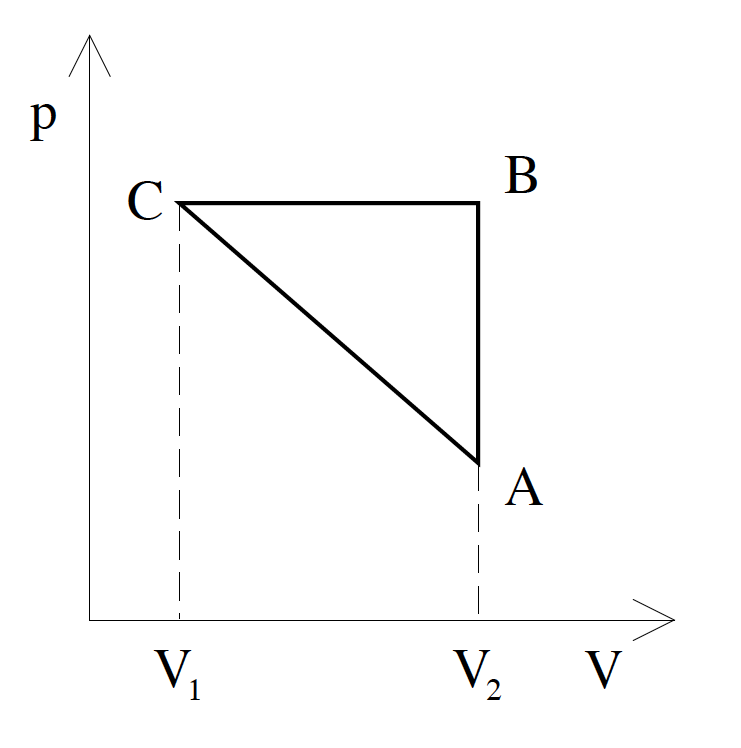
\includegraphics{seria2_rys3.png}}
\end{wrapfigure}
\zaddom
Lodówka, w której ciałem roboczym jest gaz doskonały
o cieple molowym $C_V=\frac{3}{2} R$, pracuje w cyklu przedstawionym na rysunku.
W fazie izochorycznego wzrostu ciśnienia gaz roboczy wymienia ciepło
z wnętrzem lodówki, a w pozostałych fazach wymienia ciepło z otoczeniem.
Proces $BC$ jest opisywany linią prostą we współrzędnych $p-V$.
Oblicz sprawność lodówki.

~\vspace*{1cm}
 
\begin{wrapfigure}[6]{r}{0.25\linewidth}\vspace{-5mm}
\resizebox{\linewidth}{!}{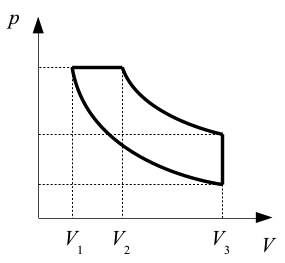
\includegraphics{seria2_rys5.png}}
\end{wrapfigure}
\zaddom
Idealny silnik cieplny pracuje w cyklu Diesla (tj. dwie adiabaty, jedna izobara, jedna izochora),
którego kontur we współrzędnych $p-V$ przedstawiony jest na rysunku.
Zaznacz właściwy kierunek cyklu.
Wyraź sprawność silnika przez stosunki objętości $V_1$, $V_2$, $V_3$.
Substancją roboczą jest gaz doskonały o cieple molowym $C_V$.\\[1mm]

%~\vspace*{1cm}
%
%\begin{wrapfigure}[6]{r}{0.275\linewidth}\vspace{-5mm}
%\resizebox{\linewidth}{!}{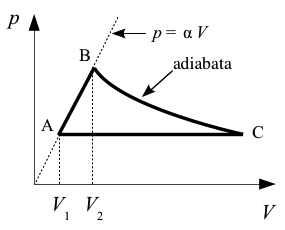
\includegraphics{seria2_rys6.png}}
%\end{wrapfigure}
%\zaddom
%Oblicz sprawność idealnego silnika cieplnego pracującego w cyklu przedstawionym
%na rysunku i wyraź ją poprzez wielkości: $\alpha$, $V_1$ i $V_2$.
%Odcinek $AB$ jest linią prostą o nachyleniu $\alpha$, zaś $BC$ jest adiabatą.
%Przyjmij, że ciałem roboczym jest jednoatomowy gaz doskonały.
%Oblicz zmianę entropii na odcinku $AB$.\\
%
%~\vspace*{1cm}
%
%\begin{wrapfigure}[6]{r}{0.3\linewidth}\vspace{0mm}
%\resizebox{\linewidth}{!}{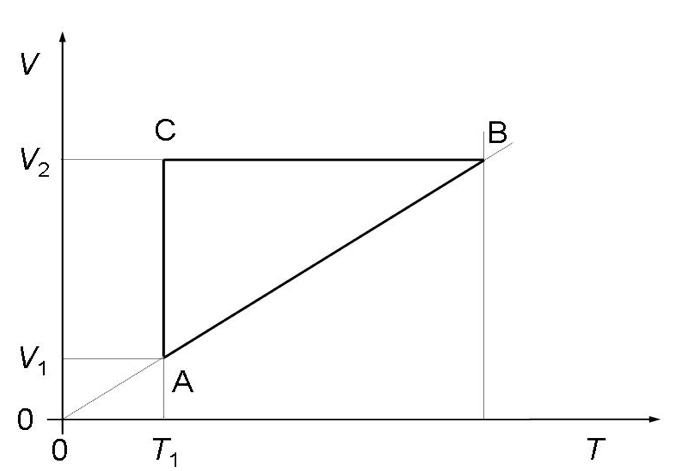
\includegraphics{seria2_rys7.png}}
%\end{wrapfigure}
%\zaddom
%Jeden mol jednoatomowego gazu doskonałego podlega przemianom
%cyklicznym przedstawionym we współrzędnych $V-T$ na rysunku obok.
%Narysuj ten cykl we współrzędnych $p-V$ i oblicz sprawność
%idealnego silnika cieplnego pracującego w takim cyklu.
%Dane są: $T_1$, $V_1$, $V_2$.\\[1mm]




% An example of figure placement:
%\begin{wrapfigure}[13]{r}{0.4\linewidth}\vspace{3mm}
%\resizebox{\linewidth}{!}{\includegraphics{NAZWA.png}}
%\end{wrapfigure}
%\zadanie

\end{document}
